% ===============================================
%                 Chapter 1B.4
%             Precipitation Reactions
%             Created by Michael Tang
%                  2025.01.03
% ===============================================

\subsubsection{1B.4 \underline{Precipitation Reactions} (沉淀反应)}
\paragraph{Overview:} Precipitation reactions involve the formation of an \underline{insoluble solid} (precipitate 沉淀) when two
solutions are mixed. They are used in chemical tests and for writing chemical equations.

\paragraph{Chemical Tests}
\begin{itemize}
    \item[1.] Carbon Dioxide
    \begin{itemize}
        \item \textbf{Test:} Bubble \ce{CO2} gas through \underline{limewater} (\ce{Ca(OH)2} 澄清石灰水).
        \item \textbf{Observation:} Limewater turns milky or cloudy due to the formation of calcium carbonate (\ce{CaCO3} 碳酸钙).
        \item \textbf{Equation:}
        \begin{equation}
            \ce{Ca(OH)2(aq) + CO2(g) -> CaCO3(s) + H2O(l)}
        \end{equation}
        \begin{figure}[H]
            \centering
            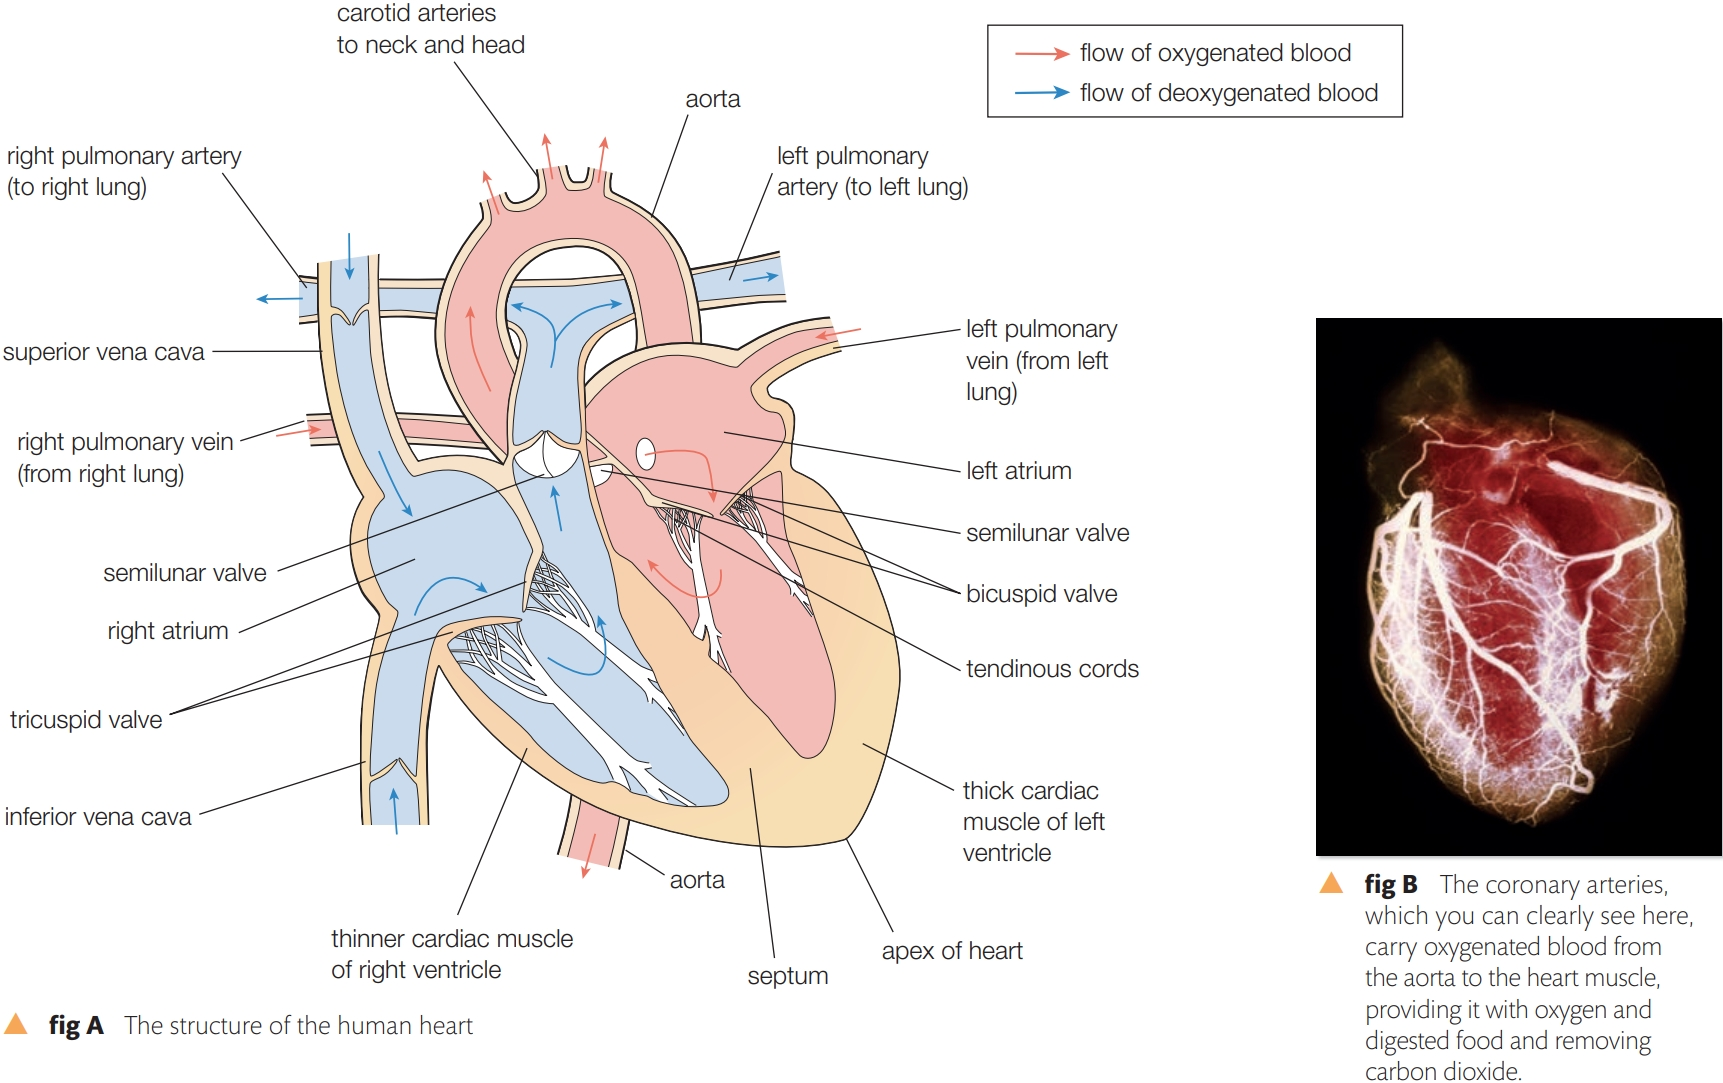
\includegraphics[scale=0.5]{Chemistry/1B/Images/1B-4-1.bmp}
            \caption{ Limewater is a colourless solution. As more carbon dioxide is bubbled through it, the amount of white
            precipitate increases.}
        \end{figure}
    \end{itemize}
    \item[2.] Sulfates
    \begin{itemize}
        \item \textbf{Test:} Add \underline{barium chloride} (\ce{BaCl2} 氯化钡) or \underline{barium nitrate} (\ce{Ba(NO3)2}
        硝酸钡) solution to a solution containing sulfate ions (\ce{SO4^2-}).
        \item \textbf{Observation:} A white precipitate of barium sulfate (\ce{BaSO4} 硫酸钡) forms.
        \item \textbf{Equation:}
        \begin{equation}
            \begin{split}
                \ce{Na2SO4(aq) + BaCl2(aq) &-> BaSO4(s) + 2NaCl(aq)}\\
                \ce{SO4^2-(aq) + Ba^2+(aq) &-> BaSO4(s)}
            \end{split}
        \end{equation}
    \end{itemize}
    \item[3.] \underline{Halides} (卤化物)
    \begin{itemize}
        \item \textbf{Test:} Add silver nitrate (\ce{AgNO3} 硝酸银) to a solution containing Halide ions (\ce{Cl-}, \ce{Br-},
        \ce{I-}).
        \item \textbf{Observation:} A precipitate of silver halide forms: White (\ce{AgCl}), Cream (\ce{AgBr}), Yellow (\ce{AgI}).
        \item \textbf{Equation:}
        \begin{equation}
            \begin{split}
                \ce{NaCl(aq) + AgNO3(aq) &-> AgCl(s) + NaNO3(aq)}\\
                \ce{Cl-(aq) + Ag+(aq) &-> AgCl(s)}
            \end{split}
        \end{equation}
    \end{itemize}
\end{itemize}

\paragraph{Working Out Equations}
Example: Reaction Between Lead Nitrate and Potassium Iodide
\begin{itemize}
    \item \textbf{Reaction:} Lead nitrate reacts with potassium iodide to form lead iodide (yellow precipitate) and potassium
    nitrate.
    \item \textbf{Word Equation:}
    \begin{equation}
        \ce{Lead Nitrate + Potassium Iodide -> Lead Iodide + Potassium Nitrate}
    \end{equation}
    \item \textbf{Balanced Equations:}
    \begin{equation}
        \begin{split}
            \ce{Pb(NO3)2(aq) + 2KI(aq) &-> PbI2(s) + 2KNO3(aq)}\\
            \ce{Pb^2+(aq) + 2I-(aq) &-> PbI2(s)}
        \end{split}
    \end{equation}
    \item Experimental Procedure:
    \begin{itemize}
        \item[1.] Place the same volume of a potassium iodide solution in a series of test tubes.
        \item[2.] Add different volumes of a lead nitrate solution to the tubes.
        \item[3.] Place each tube in a centrifuge and spin the tubes for the same length of time.
        \item[4.] Measure the depth of precipitate in each tube.
    \end{itemize}
    \item Figure 3.10 shows the results of one experiment. The concentration of both solutions is 1.0 mol dm$^{-3}$. The depth
    of each precipitate indicates the mass of precipitate formed.
    \begin{figure}[H]
        \centering
        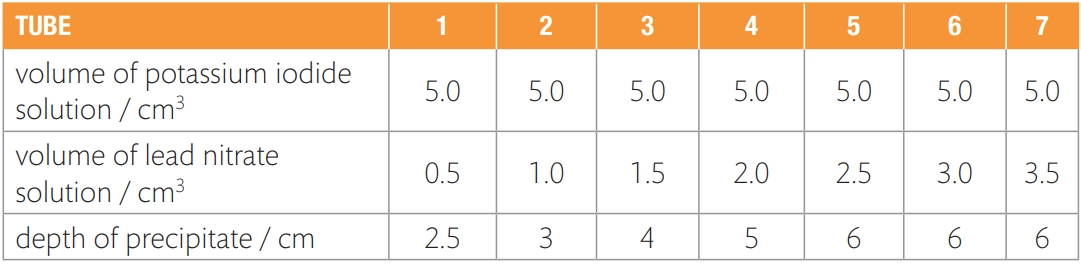
\includegraphics[scale=0.3]{Chemistry/1B/Images/1B-4-2.png}
        \caption{Results of the reaction between aqueous solutions of lead nitrate and potassium iodide in one experiment.}
    \end{figure}
    The diagram shows the tubes at the end of the experiment.
    \begin{figure}[H]
        \centering
        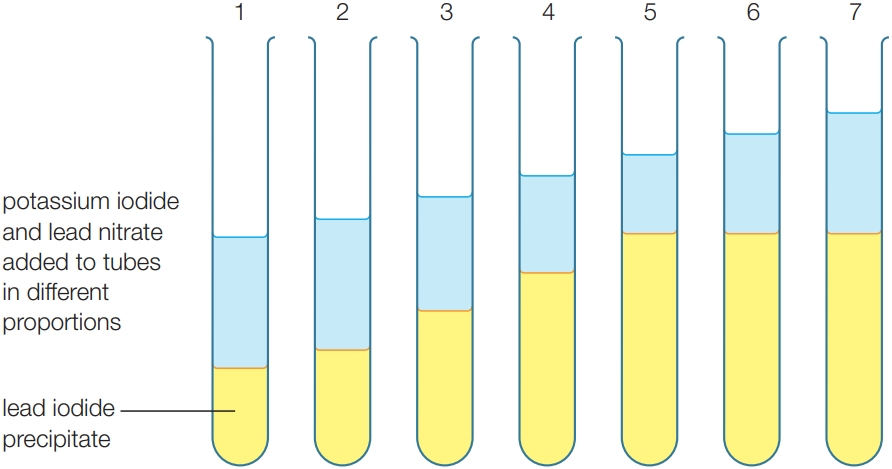
\includegraphics[scale=0.3]{Chemistry/1B/Images/1B-4-3.png}
        \caption{Results of the reaction between aqueous solutions of lead nitrate and potassium iodide in one experiment.}
    \end{figure}
    \item \textbf{Results:} Tube 5 has complete reaction with a mole ratio of lead nitrate to potassium iodide as 1:2.
    \item \textbf{Calculaton for Tube 5:}
    \begin{equation}
        \begin{split}
            n \text{(potassium iodide)} &= 0.005 \times 1.0 = 0.005 \text{mol}\\
            n \text{(lead nitrate)} &= 0.0025 \times 1.0 = 0.0025 \text{mol}
        \end{split}
    \end{equation}
\end{itemize}